
\subsection{Interpolation}

\subsubsection{Aufgaben}
Der Roboter soll in der Lage sein lineare beziehungsweise zirkulare Bewegungen durchzuführen, weshalb das Verfahren der linearen beziehungsweise zirkularen Interpolation benötigt wird. Je nach Verfahren wird eine Reihe an Zwischenpunkten berechnet, die den Start- und den Zielpunkt verbinden.

\subsubsection{Aufbau}
Um diese Aufgaben technisch umzusetzen, wurde die Klasse Interpolation entwickelt. Diese verfügt über die statischen Methoden InterpolateLinear und InterpolateCircular, welche als Ergebnis ein Objekt vom Typ InterpolationResult liefern. Da jedes Verfahren eine unterschiedliche Anzahl an Eingangsparametern übernimmt, werden diese erst in der Umsetzung näher beschrieben. Genauso wie die Kinematics-Klasse könnte diese Klasse ebenfalls in anderen, nicht roboter-bezogenen, Anwendungen verwendet werden.

\subsubsection{Umsetzung}
\textbf{InterpolationResult}\\
Die Objekt der Klasse InterpolationResult stellt, wie der Name vermuten lässt, das Ergebnis einer Interpolation dar. Da dabei viele Daten generiert werden, verfügt die Klasse über die folgenden Properties
\begin{itemize}
\item \textbf{Angles}\\
Beim Angles-Property handelt es sich um eine Liste von InterpolationStep-Objekten, welche die absoluten Winkelstellungen der Achsen an jedem berechneten Punkt enthält. 
\item \textbf{Steps}\\
Das Steps-Property stellt ebenfalls eine Liste von InterpolationStep-Objekten dar, beinhaltet jedoch die Differenz zwischen zwei Winkelstellungen. Theoretisch könnten diese auch durch Iteration durch das Angles-Property berechnet werden, jedoch würde dies zu Performance-Einbußen führen. 
\item \textbf{Points}\\
Das Points-Property stellt eine List aus Point3D-Objekten dar, welche die von der Interpolation berechneten Zwischenpunkte beinhaltet.
\item \textbf{MetaData}\\
Das MetaData-Property beinhaltet zusätzliche Informationen über den Berechnungsvorgang, wie beispielsweise Radius und Richtung der Verfahrbewegung beim zirkularen Interpolationsverfahren.
\end{itemize}
Weiters wurde die ToString-Methode überschrieben sowie die ToStepString-Methode implementiert um die Konvertierung in eine, über das Netzwerk übertragbare, Form zu erleichtern:
\begin{itemize}
\item \textbf{ToString}
Die ToString-Methode der Klasse InterpolationResult erstellt aus den Einträgen des Steps-Properties eine Zeichenfolge, deren Format auf eine einfache Interpretation durch die Steuerungssoftware der SPS ausgelegt ist. Die Einträge werden folgendermaßen konvertiert:\\
\begin{figure}[H]
  \centering
  \begin{minipage}[t]{12 cm}
  	\centering
  	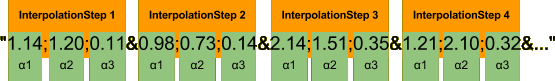
\includegraphics[width=12cm]{images/InterpolationResult} 
    \caption{Stringformat der InterpolationResult-Klasse in Winkel}
  \end{minipage}
\end{figure}
\item \textbf{ToStepString}
Die ToStepString-Methode der Klasse InterpolationResult erstellt aus den Einträgen des Steps-Properties eine Zeichenfolge, deren Format auf eine einfache Interpretation durch die Steuerungssoftware der GHI-Steuerung ausgelegt ist. Dazu müssen die individuellen Winkeländerungen in Motorschritte übersetzt werden. Die Einträge werden folgendermaßen konvertiert:\\
\begin{figure}[H]
  \centering
  \begin{minipage}[t]{12 cm}
  	\centering
  	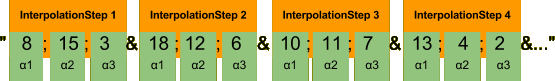
\includegraphics[width=12cm]{images/InterpolationResult2} 
    \caption{Stringformat der InterpolationResult-Klasse in Schritten}
  \end{minipage}
\end{figure}
\end{itemize}
\textbf{InterpolationStep}\\
Eine Instanz der InterpolationStep-Klasse beinhaltet Informationen zu den Winkelstellungen der Achsen an einem bestimmten Punkt. Um diese Aufgabe erfüllen zu können, sind folgende Properties definiert:
\begin{itemize}
\item \textbf{Target}\\
Das Property Target enthält jenen Punkt als \textbf{Point3D}-Objekt der mit den angegebenen Winkelstellungen erreicht wird.
\item \textbf{Alpha1}\\
Das Property Alpha1 beinhaltet die Winkelstellung der ersten Achse in Grad.
\item \textbf{Alpha2}\\
Das Property Alpha2 beinhaltet die Winkelstellung der zweiten Achse in Grad.
\item \textbf{Alpha3}\\
Das Property Alpha3 beinhaltet die Winkelstellung der dritten Achse in Grad.
\end{itemize} 
Weiters wurde auch hier die ToString-Methode überschrieben um die Konvertierung zu vereinfachen:
\begin{itemize}
\item \textbf{ToString}
Die ToString-Methode der Klasse InterpolationStep liefert die gespeicherten Informationen in folgendem Format:\\
\begin{figure}[H]
  \centering
  \begin{minipage}[t]{16.5 cm}
  	\centering
  	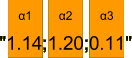
\includegraphics[width=3cm]{images/InterpolationStep} 
    \caption{Stringformat der InterpolationStep-Klasse}
  \end{minipage}
\end{figure}
\end{itemize}

\textbf{Interpolation}\\
Die Interpolations-Klasse übernimmt die Berechnung des Pfades vom Start- zum Zielpunkt. Dieser Pfad sieht je nach Verfahren unterschiedlich aus. Im Fall der linearen Interpolation handelt es sich dabei um eine Gerade, im Fall der zirkularen Interpolation um ein Kreissegment. Die Klasse definiert die Methoden InterpolateLinear und InterpolateCircular in welchen die jeweiligen Berechnungen durchgeführen und als Ergebnis ein Objekt vom Typ InterpolationResult liefern.
\begin{itemize}
\item \textbf{InterpolateLinear}\\
Die InterpolateLinear-Methode berechnet bei Aufruf eine Reihe an Winkelstellungen die nötig sind um eine lineare Bewegung vom Start zum Zielpunkt durchzuführen. Die Methode übernimmt einen Start- und einen Zielpunkt in Form eines Point3D-Objekts, sowie die Längen der beiden Achsen als float-Werte.\\
\begin{figure}[H]
  \centering
  \begin{minipage}[t]{14 cm}
  	\centering
  	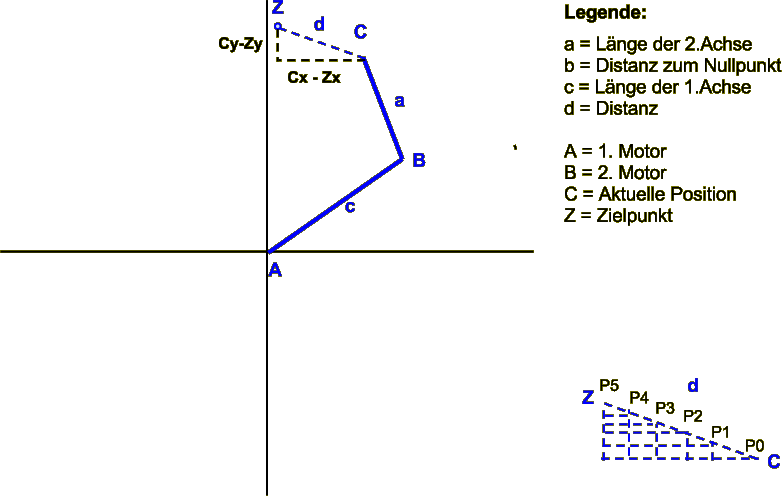
\includegraphics[width=12cm]{images/Linearinterpolation} 
    \caption{Skizze zur linearen Interpolation}
  \end{minipage}
\end{figure}
Die Vorgehensweise sieht dabei wie folgt aus:
\begin{enumerate}
\item Berechnung der Koordinaten-Differenzen:\\
Im ersten Schritt wird die Differenz zwischen den $x$-, $y$- und $z$-Koordinaten des Start- und Zielpunkts berechnet. Auf diese Differenzen wird im folgenden als $d_x$, $d_y$ und $d_z$ referenziert. 
\item Berechnung der Distanz $d$:\\
Anschließend wird die Distanz zwischen Start und Zielpunkt $d$ mit Hilfe des Satzes des Pythagoras im, durch $d_x$, $d_y$ und $d$ definierten, rechtwinkeligen Dreieck berechnet.
\begin{align*}
d = \sqrt{d_x^2+d_y^2}
\end{align*}
\item Festlegen der Schrittanzahl:\\
Mit Hilfe der Distanz wird nun die Menge an berechneten Zwischenpunkten $n$ festgelegt, welche bei unserem Verfahren dem aufgerundeten Wert von $d$ entspricht.
\item Berechnung der Steigungen:\\
Nun werden noch die Steigungen benötigt, welche festlegen um wieviel die $x$,$y$ und $z$-Koordinaten des nächsten Zwischenpunkts erhöht werden.
\begin{align*}
k_x & = \frac{d_x}{n}\\
k_y & = \frac{d_y}{n}\\
k_z & = \frac{d_z}{n}
\end{align*}
\item Berechnung der Zwischenpunkte:\\
In einer Schleife wird bei jeder Iteration die $x$-,$y$- und $z$-Koordinate des Startpunkts um die entsprechende Steigung erhöht. Daraus lassen sich die folgenden Funktionen zur Berechnung eines Zwischenpunkts ableiten:
\begin{align*}
x_n & = n k_x + x_0\\
y_n & =  n k_y + y_0\\
z_n & = n k_z + z_0 
\end{align*}
Die Winkelstellungen an einem spezifischen Zwischenpunkt werden mit Hilfe der inversen Kinematik berechnet. Das Ergebnis dieser Berechnung ist ein InterpolationStep-Objekt, welcher dem Angles-Property des InterpolationResult-Objekts hinzufügt wird. Da das Ergebnis des zuvor berechneten Punkts ebenfalls gespeichert wird, kann die Winkeldifferenz zwischen neuem und altem Punkt durch Subtraktion der InterpolationSteps berechnet werden. Dieser Wert wird dem Steps-Property des InterpolationResult-Objekt hinzufügt.
\item Rückgabe des Ergebnisses
Nachdem durch alle Zwischenpunkte iteriert wurde und das InterpolationResult-Objekt alle wichtigen Informationen aus den Berechnungen enthält, wird dieses an die aufrufende Methode zurückgegeben.
\end{enumerate}
\item \textbf{InterpolateCircular}\\
Die InterpolateCircular-Methode berechnet bei Aufruf eine Reihe an Winkelstellungen die nötig sind um eine zirkulare Bewegung vom Start zum Zielpunkt durchzuführen. Die Methode übernimmt einen Start-, einen Mittel- und einen Zielpunkt in Form eines Point3D-Objekts, sowie die Längen der beiden Achsen als float-Werte. Der Mittelpunkt legt fest wie scharf die Kurve vom Start- zum Zielpunkt ist.\\
\begin{figure}[H]
  \centering
  \begin{minipage}[t]{14 cm}
  	\centering
  	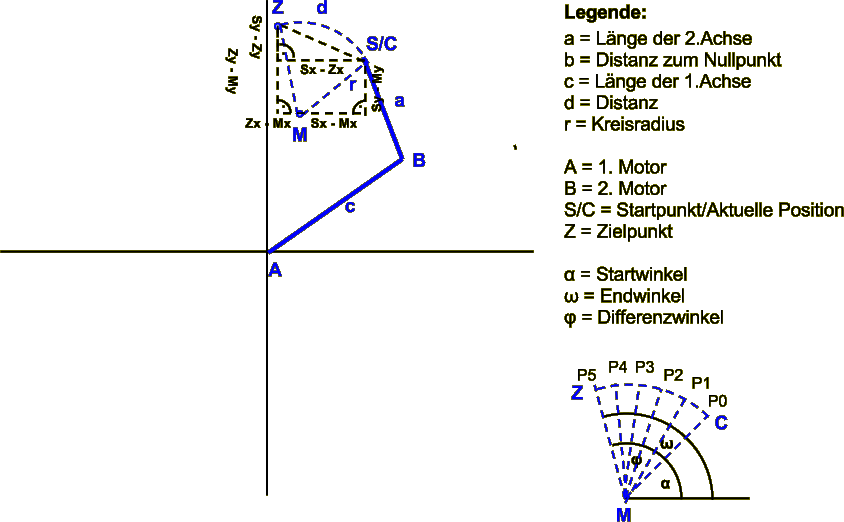
\includegraphics[width=12cm]{images/Zirkularinterpolation} 
    \caption{Skizze zur zirkularen Interpolation}
  \end{minipage}
\end{figure}
Die Vorgehensweise sieht dabei wie folgt aus:
\begin{enumerate}
\item Prüfung des Start- und Zielpunkts\\
Bevor mit der Berechnung der Bahn begonnen werden kann, muss geprüft werden ob sich Start- und Zielpunkt überhaupt Teil des durch den Mittelpunkt angegebenen Kreises liegt. Dazu wird jeweils die Differenz zwischen Mittelpunkt $M$ und dem Startpunkt $S$ beziehungsweise Zielpunkt $Z$ berechnet. Dazu werden die jeweiligen Distanzen zwischen den $x$- und $y$-Koordinaten verwendet und mit Hilfe dieser die Gesamtdistanz berechnet.
\begin{align*}
d_{\overrightarrow{MS}} & = \sqrt{d_{x\overrightarrow{MS}}^2 + d_{y\overrightarrow{MS}}^2}\\
d_{\overrightarrow{MZ}} & = \sqrt{d_{x\overrightarrow{MZ}}^2 + d_{y\overrightarrow{MZ}}^2}
\end{align*}
Sind diese Werte gleich, so stellen sie den Kreisradius $r$ dar und beweisen, dass beide Punkte sich am Kreisrand befinden, andernfalls wird eine MVCException ausgelöst und die Berechnung abgebrochen. 
\item Berechnung der Distanz $d_{\overrightarrow{SZ}}$\\
Nun wird noch die Distanz zwischen Start- und Zielpunkt $d$, erneut mit Hilfe der $x$- beziehungsweise $y$-Differenz und dem Satz des Pythagoras, berechnet.
\begin{align*}
d_{\overrightarrow{SZ}} = \sqrt{d_{x\overrightarrow{SZ}}^2 + d_{y\overrightarrow{SZ}}^2}
\end{align*}
%\item Berechnung des Differenzwinkels $\varphi$:\\
%Mit Hilfe des entstandenen, gleichschenkeliges Dreieck, welches durch $d_{\overrightarrow{SZ}}$ und $r$ definiert wird, können wir den Differenzwinkel $\varphi$ zwischen Start- und Zielpunkt berechnen. Dieser wird mit Hilfe des umgeformten %Kosinussatzes berechnet. Auf unsere Variablen angepasst sieht die Formel für die Berechnung des Winkels $\varphi$ folgendermaßen aus:
%\begin{align*}
%d_{\overrightarrow{SZ}}^2 & = r^2 + r^2 - 2rr \cos \varphi \\
%d_{\overrightarrow{SZ}}^2 & = 2r^2 - 2r^2 \cos \varphi \\
%d_{\overrightarrow{SZ}}^2 & = 2r^2(1 - \cos \varphi) \\
%\frac{d_{\overrightarrow{SZ}}^2}{2r^2} & = 1 - \cos \varphi \\
%\cos \varphi & = 1 - \frac{d_{\overrightarrow{SZ}}^2}{2r^2} \\
%\varphi & = \arccos (1 - \frac{d_{\overrightarrow{SZ}}^2}{2r^2})
%\end{align*}
\item Berechnung des Startwinkels $\alpha$:\\
Da der Startpunkt in Bezug auf den Mittelpunkt nicht zwingend bei 0$^\circ$ liegen muss, wird der sogenannte Startwinkel $\alpha$ mit dem Kosinus im rechtwinkeligen Dreieck berechnet. Das verwendete Dreieck ist durch die $x$ und $y$-Differenz zwischen Start- und Mittelpunkt, sowie den Radius $r$ definiert.
\item Berechnung des Endwinkels $\omega$:
Zuerst wird jener Winkel berechnet, zwischen 0$^\circ$ und dem Zielpunkt liegt.
\begin{align*}
\cos \omega & = \frac{d_{x\overrightarrow{MZ}}}{r}\\
\omega & = \arccos \frac{d_{x\overrightarrow{MZ}}}{r}
\end{align*}
\item Überprüfung der Quadranten\\
Aufgrund der Tatsache, dass die Arkussinus-Funktion in beiden Fällen lediglich einen Winkel zwischen 0$^\circ$ und 180$^\circ$ liefert, muss der Quadrant in dem sich der Start beziehungsweise der Zielpunkt befindet überprüft werden. Befindet einer dieser Punkte  im 3. oder 4. Quadranten so wird Vorzeichen des entsprechenden Winkels, $\alpha$ beim Startpunkt beziehungsweise $\omega$ beim Zielpunkt, umgedreht. 
\item Berechnung des Differenzwinkels $\varphi$:\\
Mit Hilfe des Start und des Endwinkels kann nun der zu verfahrende Winkel berechnet werden.
\begin{align*}
\varphi = \omega - \alpha
\end{align*}
\item Berechnung der Bogenlänge $s$:
Mit dem Differenzwinkel $\varphi$ wird die tatsächliche Wegsstrecke, die Bogenlänge $s$, berechnet.
\begin{align*}
s = \frac{2r \pi \varphi}{360}
\end{align*}
\begin{align*}
\cos \alpha & = \frac{d_{x\overrightarrow{MS}}}{r}\\
\alpha & = \arccos \frac{d_{x\overrightarrow{MS}}}{r}
\end{align*}
\item Festlegen der Schrittanzahl:\\
Mit Hilfe der Bogenlänge $s$ wird nun die Menge an berechneten Zwischenpunkten $n$ festgelegt, welche bei unserem Verfahren dem aufgerundeten Wert von  $s$ entspricht.
\item Berechnung der Winkelsteigung:\\
Nun wird der Differenzwinkel $\varphi$ durch die Schrittanzahl $n$ dividiert um die Winkelsteigung zu erhalten, welche nach jedem berechneten Zwischenpunkt zum Startwinkel addiert wird.
\begin{align*}
k & = \frac{\varphi}{n}
\end{align*}
\item Berechnung der Zwischenpunkte:\\
In einer Schleife wird bei jeder Iteration die Winkelsteigung zum Startwinkel addiert und anschließend mit Hilfe desselben, in Punkt 5 beschriebenen, rechtwinkeligen Dreiecks berechnet. Die gesuchte $x$ beziehungsweise $y$-Koordinate des nächsten Zwischenpunkts wird über die Sinus- beziehungsweise Kosinusfunktion berechnet und zu der entsprechenden Koordinate des Mittelpunkts addiert.
\begin{align*}
\cos \alpha & = \frac{x}{r} & \sin \alpha & = \frac{y}{r}\\
x & = r \cos \alpha & y & = r \cos \alpha
\end{align*}
Die Winkelstellungen an einem spezifischen Zwischenpunkt werden mit Hilfe der inversen Kinematik berechnet. Das Ergebnis dieser Berechnung ist ein InterpolationStep-Objekt, welcher dem Angles-Property des InterpolationResult-Objekts hinzufügt wird. Da das Ergebnis des zuvor berechneten Punkts ebenfalls gespeichert wird, kann die Winkeldifferenz zwischen neuem und altem Punkt durch Subtraktion der InterpolationSteps berechnet werden. Dieser Wert wird dem Steps-Property des InterpolationResult-Objekt hinzufügt.
\item Rückgabe des Ergebnisses
Nachdem durch alle Zwischenpunkte iteriert wurde und das InterpolationResult-Objekt alle wichtigen Informationen aus den Berechnungen enthält, wird dieses an die aufrufende Methode zurückgegeben.
\end{enumerate}
\end{itemize}